\subsection{Variasi Pengujian}

\subsubsection{Variasi Sistem Tiket}

Terdapat empat variasi sistem yang akan diuji pada penelitian ini, yaitu:

\begingroup
\footnotesize
\begin{longtable}{|l|l|l|}
    \caption{Variasi Sistem Selama Pengujian}                                                 \\
    \hline
    \textbf{ID}   & \textbf{Pengendalian Aliran} & \textbf{Basis Data}                        \\
    \hline
    \endfirsthead

    \multicolumn{3}{|l|}{\tablename\ \thetable\ -- \textit{Lanjutan dari halaman sebelumnya}} \\
    \hline
    \textbf{ID}   & \textbf{Pengendalian Aliran} & \textbf{Basis Data}                        \\
    \hline
    \endhead

    \hline
    \multicolumn{3}{|r|}{\textit{Dilanjutkan ke halaman berikutnya}}                          \\
    \endfoot

    \hline
    \endlastfoot

    nofc-pg       & Tidak                        & PostgreSQL                                 \\
    \hline
    nofc-citus    & Tidak                        & CitusData                                  \\
    \hline
    nofc-yugabyte & Tidak                        & YugabyteDB                                 \\
    \hline
    fc-pg         & Ya                           & PostgreSQL                                 \\
    \hline
\end{longtable}
\endgroup

Varian nofc-pg merupakan varian yang menjadi tolok ukur/basis pengujian untuk mengukur kinerja varian yang lain.

\pagebreak

\subsubsection{Variasi Skenario Penjualan Tiket}

Terdapat dua skenario yang akan digunakan selama pengujian, yaitu:

\begin{enumerate}
    \item Skenario penjualan sf-4, yaitu skenario skala penuh (80.000 tiket per hari) yang diselenggarakan selama 4 hari. Total tiket yang dijual adalah 320.000 tiket.
    \item Skenario penjualan s10-2, yaitu skenario skala satu berbanding sepuluh (8.000 tiket per hari) yang diselenggarakan selama 2 hari. Total tiket yang dijual adalah 16.000 tiket.
\end{enumerate}

\subsection{Skenario Pengujian}

Terdapat dua skenario pengujian yang dilakukan, yaitu skenario beban berkelanjutan dan skenario perebutan tiket. Banyaknya pengguna dalam satu waktu (\textit{concurrent user}) didefinisikan sebagai VU (\textit{virtual user}). Satu iterasi berarti satu alur eksekusi penuh simulasi pengguna. Terdapat perbedaan mendasar pada kedua skenario. Skenario beban berkelanjutan menjaga agar \textit{concurrent user} tetap sama sepanjang waktu, sedangkan skenario perebutan tiket menggunakan distribusi \textit{arrival} pengguna sehingga jumlah \textit{concurrent user} tidak selalu sama.

Berikut adalah daftar skenario pengujian beban berkelanjutan:

\begingroup
\footnotesize
\begin{longtable}{|l|l|l|l|l|}
    \caption{Skenario Beban Berkelanjutan}                                                                                  \\
    \hline
    \textbf{ID} & \textbf{Skenario Penjualan} & \textbf{Jumlah Iterasi} & \textbf{Banyaknya VUs} & \textbf{Durasi Maksimal} \\
    \hline
    \endfirsthead

    \multicolumn{5}{|l|}{\tablename\ \thetable\ -- \textit{Lanjutan dari halaman sebelumnya}}                               \\
    \hline
    \textbf{ID} & \textbf{Skenario Penjualan} & \textbf{Jumlah Iterasi} & \textbf{Banyaknya VUs} & \textbf{Durasi Maksimal} \\
    \hline
    \endhead

    \hline
    \multicolumn{5}{|r|}{\textit{Dilanjutkan ke halaman berikutnya}}                                                        \\
    \endfoot

    \hline
    \endlastfoot

    stress-2    & sf-4                        & 350.000                 & 10.000                 & 15 menit                 \\
    \hline
    stress-1    & sf-4                        & 350.000                 & 12.000                 & 15 menit                 \\
    \hline
    stress-0    & sf-4                        & 350.000                 & 15.000                 & 10 menit                 \\
    \hline
\end{longtable}
\endgroup

Berikut adalah daftar skenario pengujian perebutan tiket:

\begingroup
\footnotesize
\begin{longtable}{|l|l|l|l|l|}
    \caption{Skenario Perebutan Tiket}                                                                                   \\
    \hline
    \textbf{ID} & \textbf{Skenario Penjualan} & \textbf{Jumlah Iterasi} & \textbf{VUs Puncak} & \textbf{Durasi Maksimal} \\
    \hline
    \endfirsthead

    \multicolumn{4}{|l|}{\tablename\ \thetable\ -- \textit{Lanjutan dari halaman sebelumnya}}                            \\
    \hline
    \textbf{ID} & \textbf{Skenario Penjualan} & \textbf{Jumlah Iterasi} & \textbf{VUs Puncak} & \textbf{Durasi Maksimal} \\
    \hline
    \endhead

    \hline
    \multicolumn{5}{|r|}{\textit{Dilanjutkan ke halaman berikutnya}}                                                     \\
    \endfoot

    \hline
    \endlastfoot

    sim-1       & s10-2                       & 40.000                  & 15.000              & 10 menit                 \\
\end{longtable}
\endgroup

Kedatangan pengguna skenario perebutan tiket mengikuti distribusi lognormal yang digambarkan pada grafik berikut:

\begin{figure}[htbp]
    \centering
    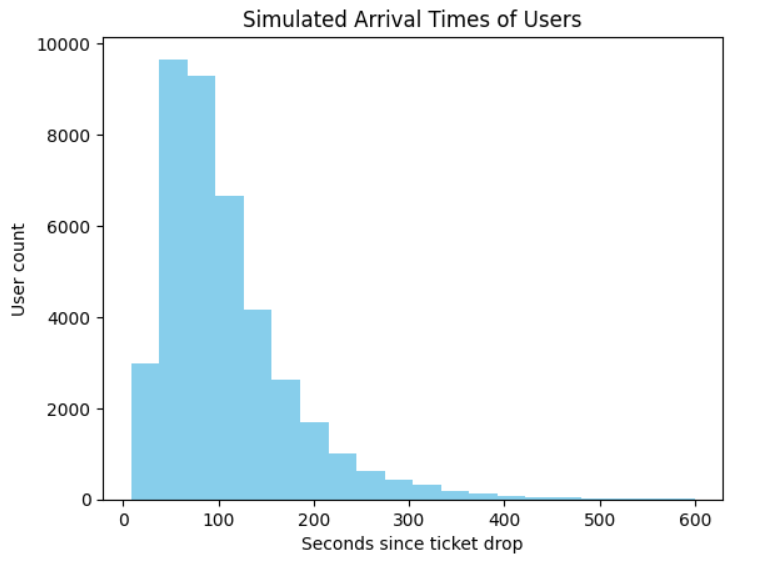
\includegraphics[width=1\textwidth]{resources/chapter-4/arrival-sim.png}
    \caption{Distribusi Kedatangan Pengguna Skenario Perebutan Tiket}
    \label{fig:vus-arrival}
\end{figure}

Skenario pengujian berfokus pada pengujian dengan beban berkelanjutan. Hal ini agar berfokus agar sistem dapat menjalankan skenario penjualan dengan skala penuh dan sistem secara konsisten berada pada beban yang sama selama waktu pengujian. Meskipun begitu, distribusi beban sesungguhnya sistem ini memiliki distribusi kedatangan yang serupa dengan skenario pengujian perebutan tiket. Agar pengujian dapat dilakukan dengan skenario penjualan yang lebih banyak dengan rasio distribusi kedatangan yang sama, kluster penguji harus mampu menangani jumlah \textit{concurrent user} yang jauh lebih banyak. Hal ini berarti kebutuhan sumber daya untuk kluster pengujian menjadi semakin tinggi. Selain itu, estimasi kebutuhan sumber daya akan menjadi lebih sulit karena jumlah \textit{concurrent user} sangat dinamis karena kemampuan sistem menangani permintaan pengguna berbeda-beda. Selama eksperimen, kluster penguji hanya mampu menangani jumlah \textit{concurrent user} sebanyak 15.000 VUs.
